% \begin{frame}{Visualization: What do those networks learn?}
%   \note{
%     \begin{itemize}
%       \item The black box!?
%       \item
%     \end{itemize}
%   }
% \end{frame}


\begin{frame}{Visualization: Filters}
      \begin{figure}
        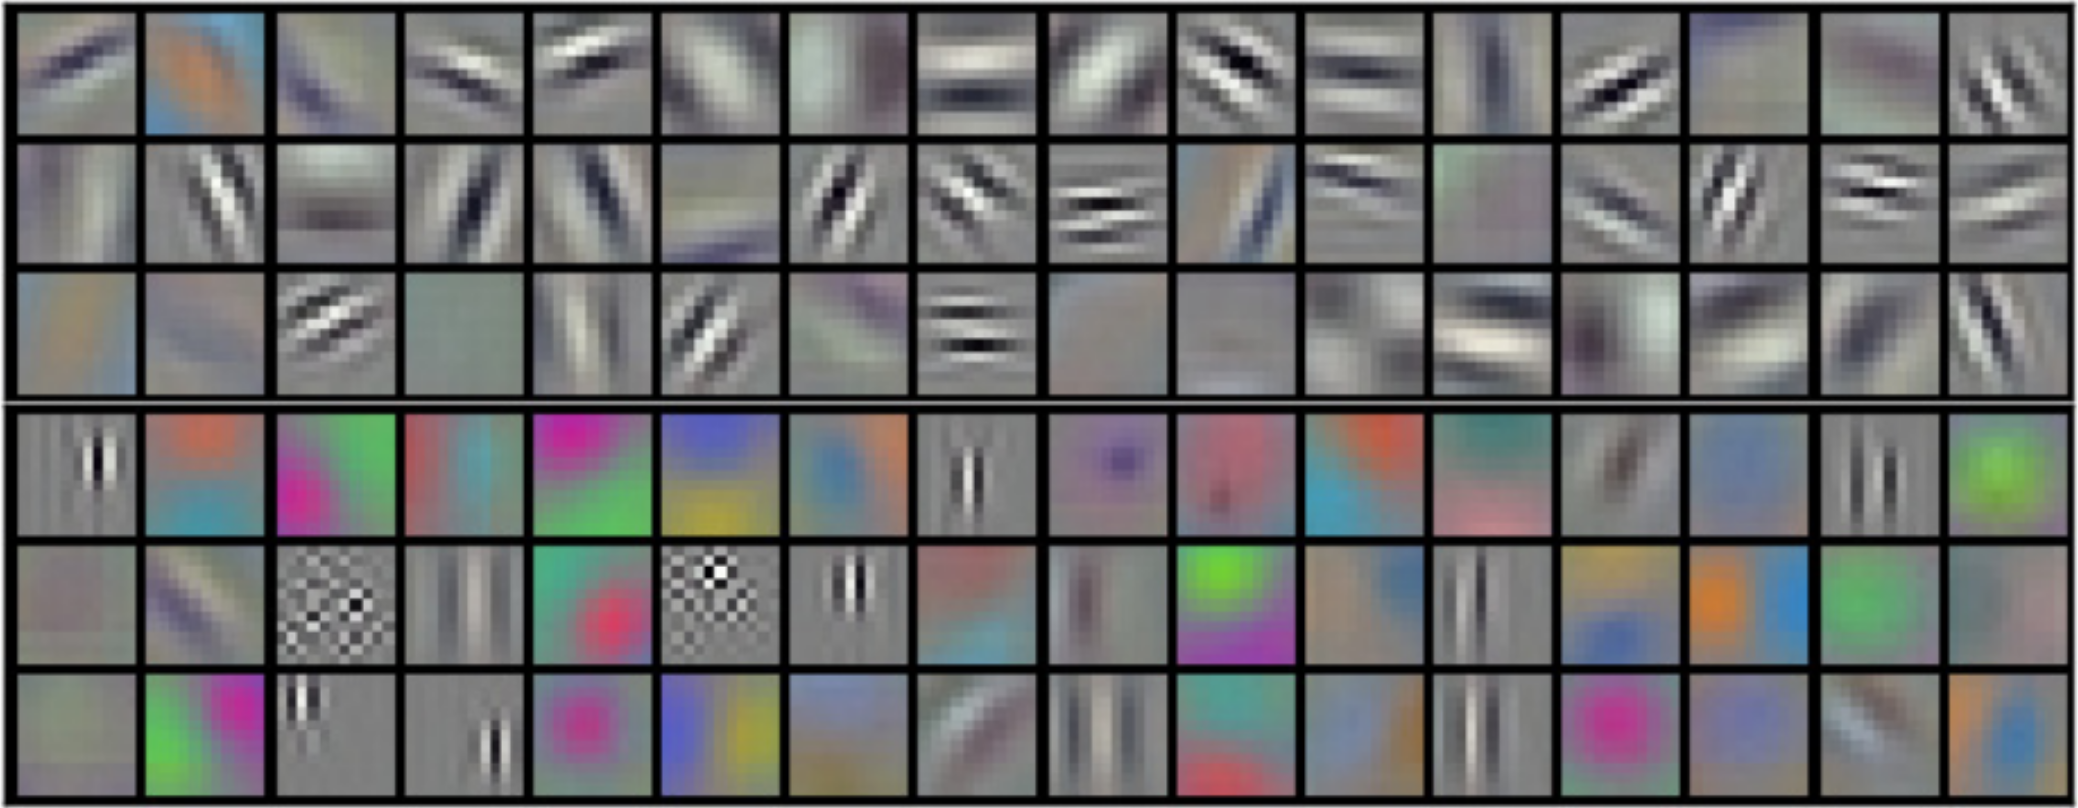
\includegraphics[width=0.9\textwidth]{alexnet_filters}
      \end{figure}

  \note{
    \begin{itemize}
      \item Filters of the first convolutional layer in AlexNet.
      \item ImageNet Classification with Deep Convolutional Neural Networks, Krizhevsky et al, NeurIPS 2012
    \end{itemize}
  }
\end{frame}


\begin{frame}{Visualization: Early}

  \begin{columns}
    \begin{column}{0.1\textwidth}
      \begin{figure}
        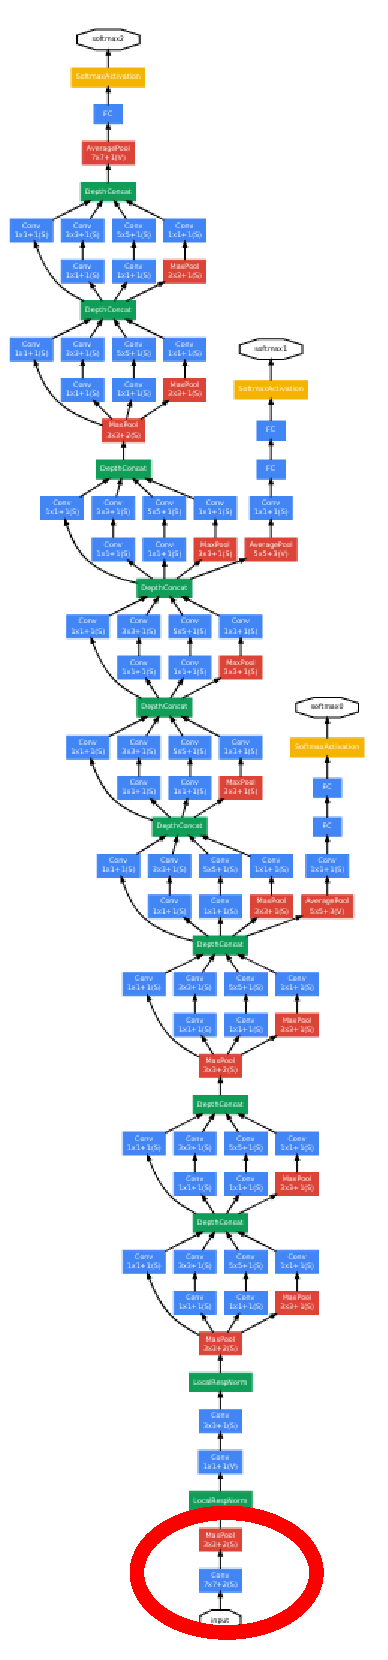
\includegraphics[width=0.9\textwidth]{visualize_00}
      \end{figure}
    \end{column}
    \begin{column}{0.9\textwidth}
      \begin{figure}
        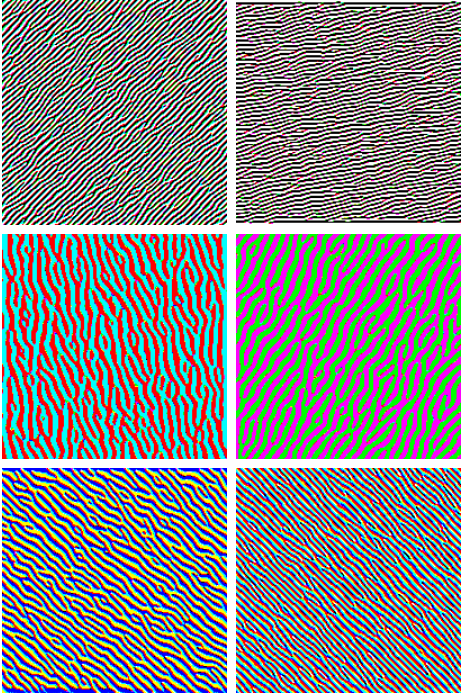
\includegraphics[width=0.4\textwidth]{fvis_conv_00}
      \end{figure}
    \end{column}
  \end{columns}

  \note{
    \begin{itemize}
      \item Going deeper with convolutions, Szegedy et al, CVPR 2015
      \item Feature Visualization, Olah et al, https://distill.pub/2017/feature-visualization/
    \end{itemize}
  }
\end{frame}


\begin{frame}{Visualization: Middle}

  \begin{columns}
    \begin{column}{0.1\textwidth}
      \begin{figure}
        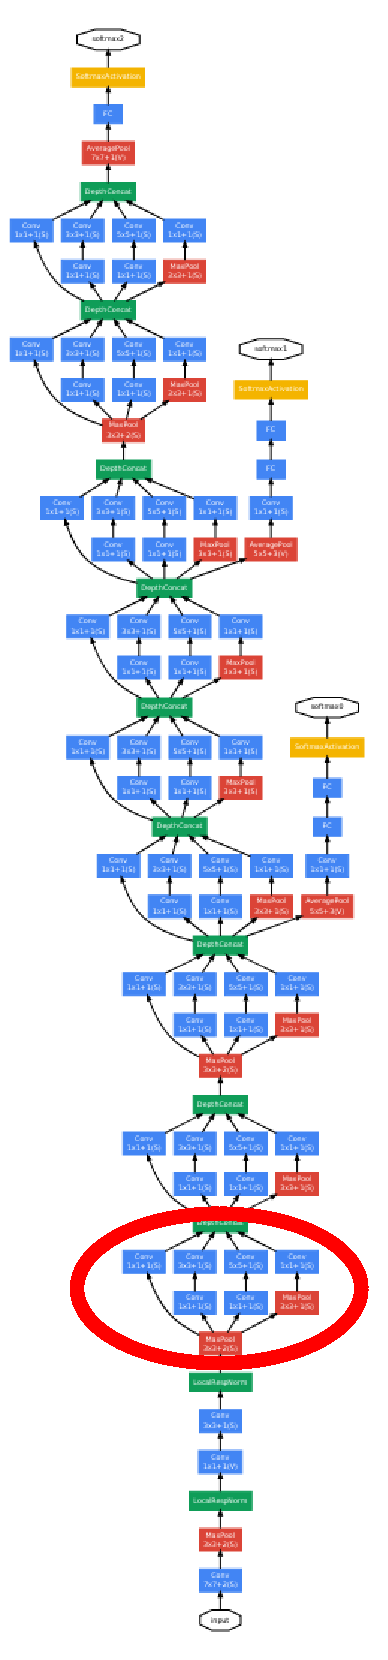
\includegraphics[width=0.9\textwidth]{visualize_01}
      \end{figure}
    \end{column}
    \begin{column}{0.9\textwidth}
      \begin{figure}
        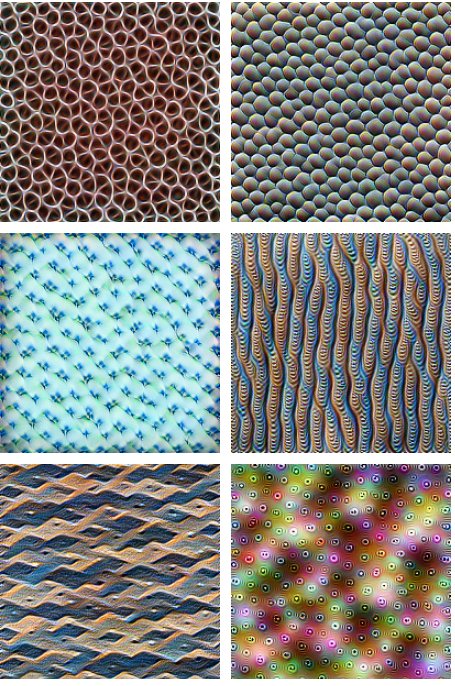
\includegraphics[width=0.4\textwidth]{fvis_mixed3a}
      \end{figure}
    \end{column}
  \end{columns}

  \note{
    \begin{itemize}
      \item
      \item
    \end{itemize}
  }
\end{frame}


\begin{frame}{Visualization: Middle}

  \begin{columns}
    \begin{column}{0.1\textwidth}
      \begin{figure}
        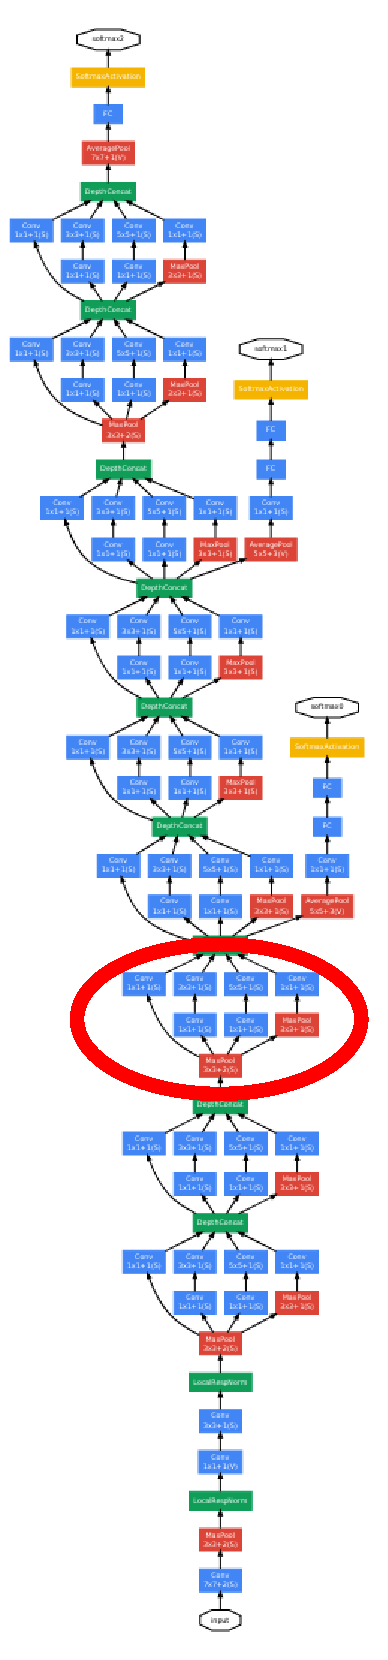
\includegraphics[width=0.9\textwidth]{visualize_02}
      \end{figure}
    \end{column}
    \begin{column}{0.9\textwidth}
      \begin{figure}
        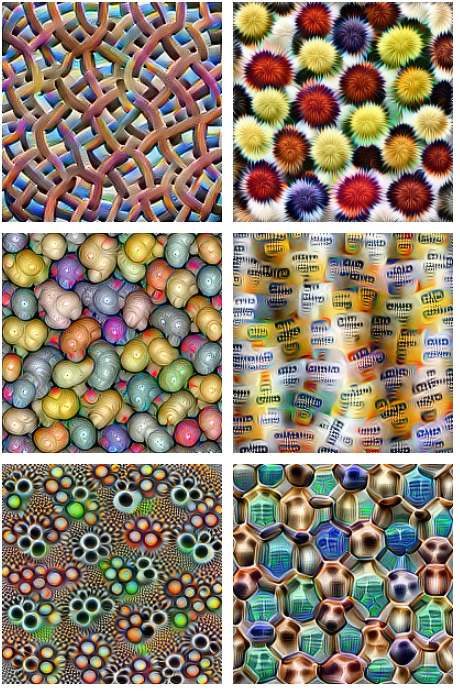
\includegraphics[width=0.4\textwidth]{fvis_mixed4a}
      \end{figure}
    \end{column}
  \end{columns}

  \note{
    \begin{itemize}
      \item
      \item
    \end{itemize}
  }
\end{frame}


\begin{frame}{Visualization: Middle}

  \begin{columns}
    \begin{column}{0.1\textwidth}
      \begin{figure}
        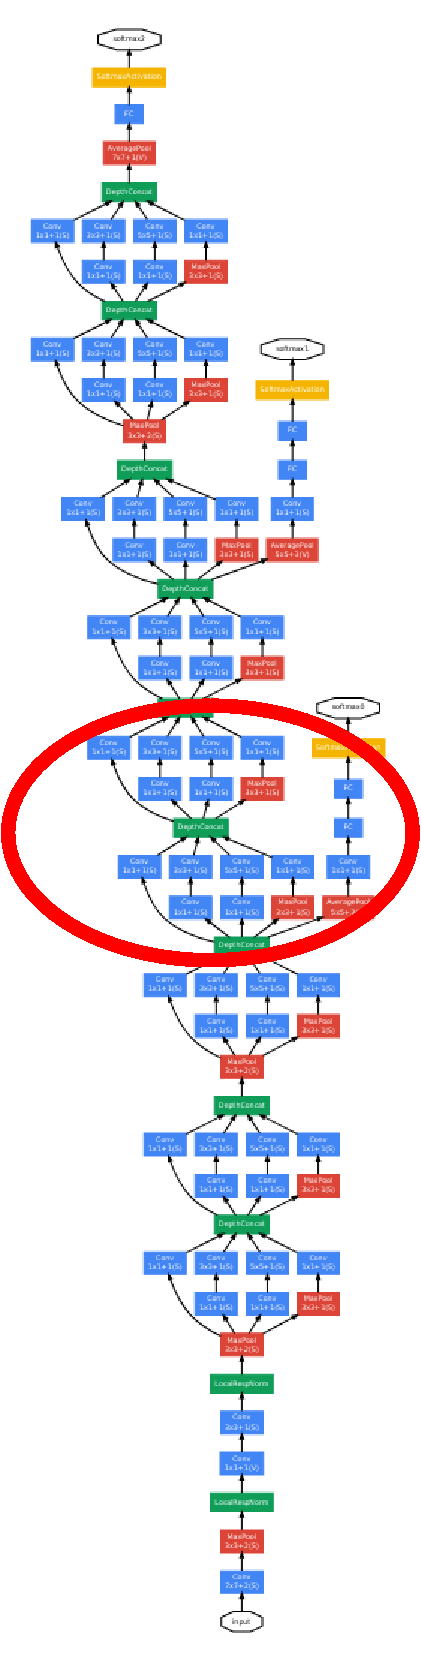
\includegraphics[width=0.9\textwidth]{visualize_03}
      \end{figure}
    \end{column}
    \begin{column}{0.9\textwidth}
      \begin{figure}
        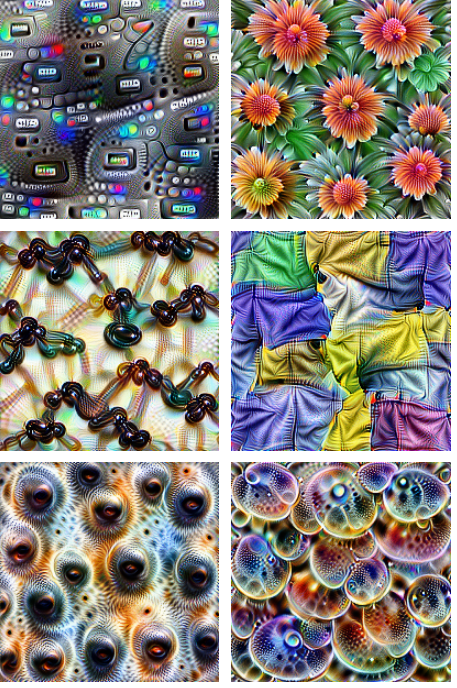
\includegraphics[width=0.4\textwidth]{fvis_mixed4bc}
      \end{figure}
    \end{column}
  \end{columns}

  \note{
    \begin{itemize}
      \item
      \item
    \end{itemize}
  }
\end{frame}



\begin{frame}{Visualization: Late}

  \begin{columns}
    \begin{column}{0.1\textwidth}
      \begin{figure}
        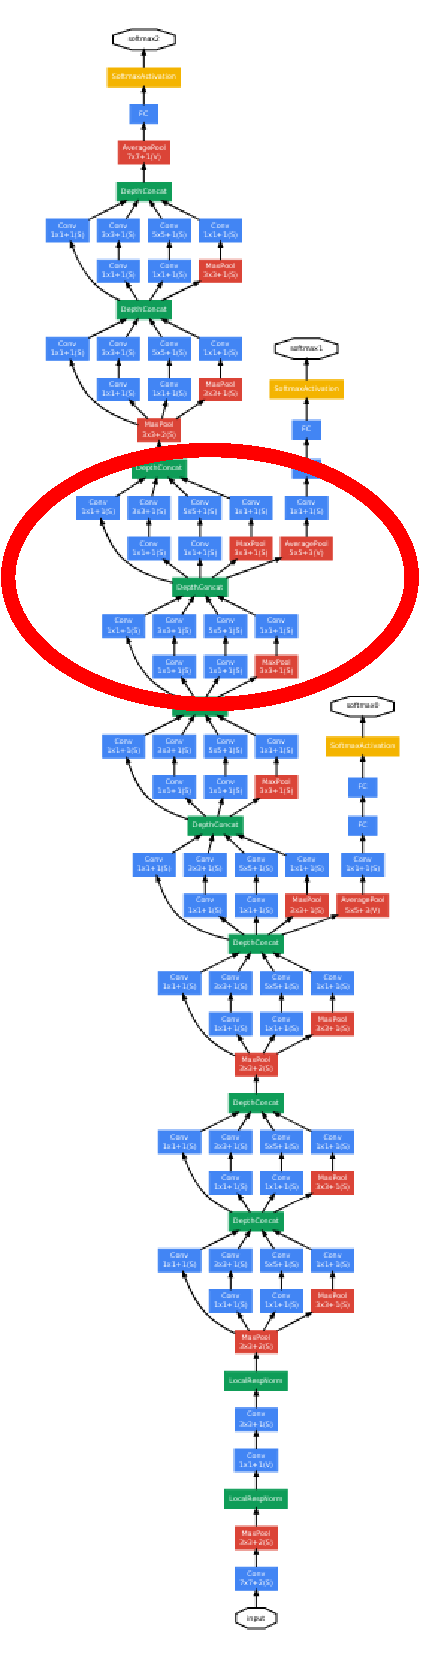
\includegraphics[width=0.9\textwidth]{visualize_04}
      \end{figure}
    \end{column}
    \begin{column}{0.9\textwidth}
      \begin{figure}
        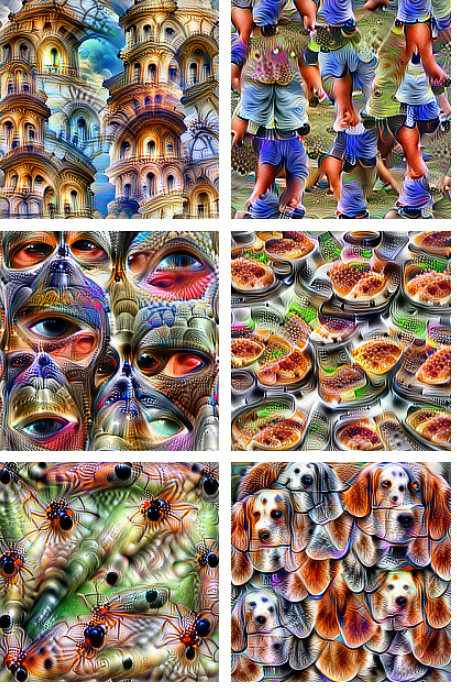
\includegraphics[width=0.4\textwidth]{fvis_mixed4de}
      \end{figure}
    \end{column}
  \end{columns}

  \note{
    \begin{itemize}
      \item
      \item
    \end{itemize}
  }
\end{frame}
